% !TEX root = ../thesis.tex
\chapter{Approach}
\label{ch:approach}
% **************************** Define Graphics Path **************************
\ifpdf
\graphicspath{{Chapter3/Figs/Raster/}{Chapter3/Figs/PDF/}{Chapter3/Figs/}}
\else
\graphicspath{{Chapter3/Figs/Vector/}{Chapter3/Figs/}}
\fi

\section{Introduction}
\label{sec:approachIntro}
Despite the importance of crowd monitoring in mass gathering events, the literature review in the previous chapter is able to identify several gaps in the research, especially in crowd modelling. Most state-of-art crowd monitoring techniques do not incorporate a typology to distinguish different types of crowd. In other words, no explicit type of crowd is defined in those approaches.

say something more about crowd modelling

conclude with the need of a crowd monitoring framework

\section{An Overview of the Crowd Monitoring Framework}

The literature review in Chapter \ref{ch:litReview} has summarised that most of the state-of-art crowd monitoring approaches are focusing on using computer vision to automate the analysis of CCTV system. The literature review has also noted several limitations of the computer vision technique, such as the effect of obstacles and low lighting condition. With the rapid development of mobile computing and the increasing popularity of mobile devices, mobile sensing seems to be a more potential technique to collect contextual data for crowd monitoring. Information about the context are obtained from a variety of sensors integrated in mobile phones and wearable devices, for example GPS receivers and accelerometers. Apart from those ``hard sensors'', the literature review also highlights that another type of information source known as the ``soft sensor'' can be used to monitor the peace of a crowd, which is the social media. The use of social media analysis for crowd monitoring has been introduced in a related work by \citet{DelirHaghighi2013}. It has the great advantage of feasibility as it only relies on the software and no additional hardware is required to be installed. Despite this strength, our literature review shows that very limited works have been done to utilize social media to support emergency management.

Secondly, another finding from the literature review is that emotions are one of the key factors that form and motivate collective behaviours, which in our context are the crowd behaviours. Hence, it is essential for a crowd monitoring approach to consider the influence of emotions in the crowd. Although human emotion is an abstract concept and very difficult to measure with ``hard sensors'', it is very possible to capture the emotion of a person from the verbal expressions, such as writing or voice. This is where social media further proves its advantage over the ``hard sensors''. By applying analysis on the social media, we can capture the emotions in a crowd, thus enabling the inference of the crowd's condition. For that reason, in this project, we would like to propose a crowd monitoring framework that employs the emotion analysis of social media to support emergency management in mass gatherings. 

Finally, our literature review also reveals another gap in the research that is the lack of a crowd model that can distinguish different crowd types. Most existing crowd monitoring techniques do not base on any model thus making it difficult to identify exactly what crowd type is happening without the interpretation of human. By exploring broader into other disciplines, our literature review is able to point out several notable works on crowd modelling and classification in the police literature and public safely science. Among those works, Berlonghi's wowrk stands out as the most commonly adopted model by the emergency management bureaus worldwide. Our proposed crowd monitoring framework is established on the Berlonghi's model which consists of eleven different crowd types. Yet, a systematic approach to classify one crowd into those types is challenging because Berlonghi's model only describes the crowd types and there is no attribute defined in the existing model. Therefore, in our approach, we would like to propose a mapping model that connects the emotion model with crowd model, enabling the the fuzzy classification of crowd type by emotions.

In conclusion, our proposed approach will address the gaps that are identified in the previous chapters by: 
\begin{inparaenum}[i)]
\item incorporating social media as the information source for context data;
\item capturing the emotions of a crowd by analysing the context data;
\item identifying the type of a crowd by applying fuzzy inference to the crowd emotions
\end{inparaenum}. These objectives can be integrated together in a complete process as illustrated by Figure \ref{fig:processOverview}. Social media is firstly probed to get the context data at the raw level. This raw data is then processed in an emotion analysis to extract high level context data, that is the emotional states of the crowd. These emotional states are in turn used as the attributes or features to classify a crowd into a specific type.

\begin{figure}[htbp!] 
\centering    
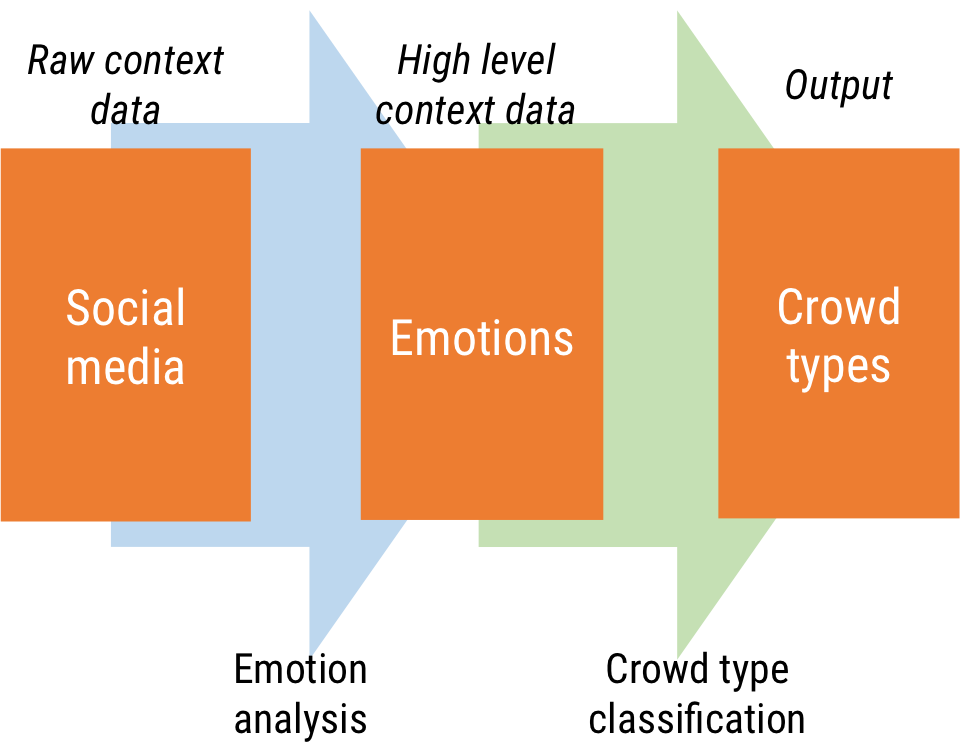
\includegraphics[width=1.0\textwidth]{ProcessOverview}
\caption{A process to identify a crowd type from social media}
\label{fig:processOverview}
\end{figure}

From functional point of view, the process can be implemented into a framework. Figure \ref{fig:frameworkOverview} shows our framework consisting of following components:
\begin{inparaenum}[i)]
\item Context data;
\item Emotion analysis;
\item Emotion model;
\item Crowd model;
\item Emotion - Crowd type mapping model;
\item Rule based reasoning
\end{inparaenum}. Each component will be discussed further in the sections below.

\begin{figure}[htbp!] 
\centering    
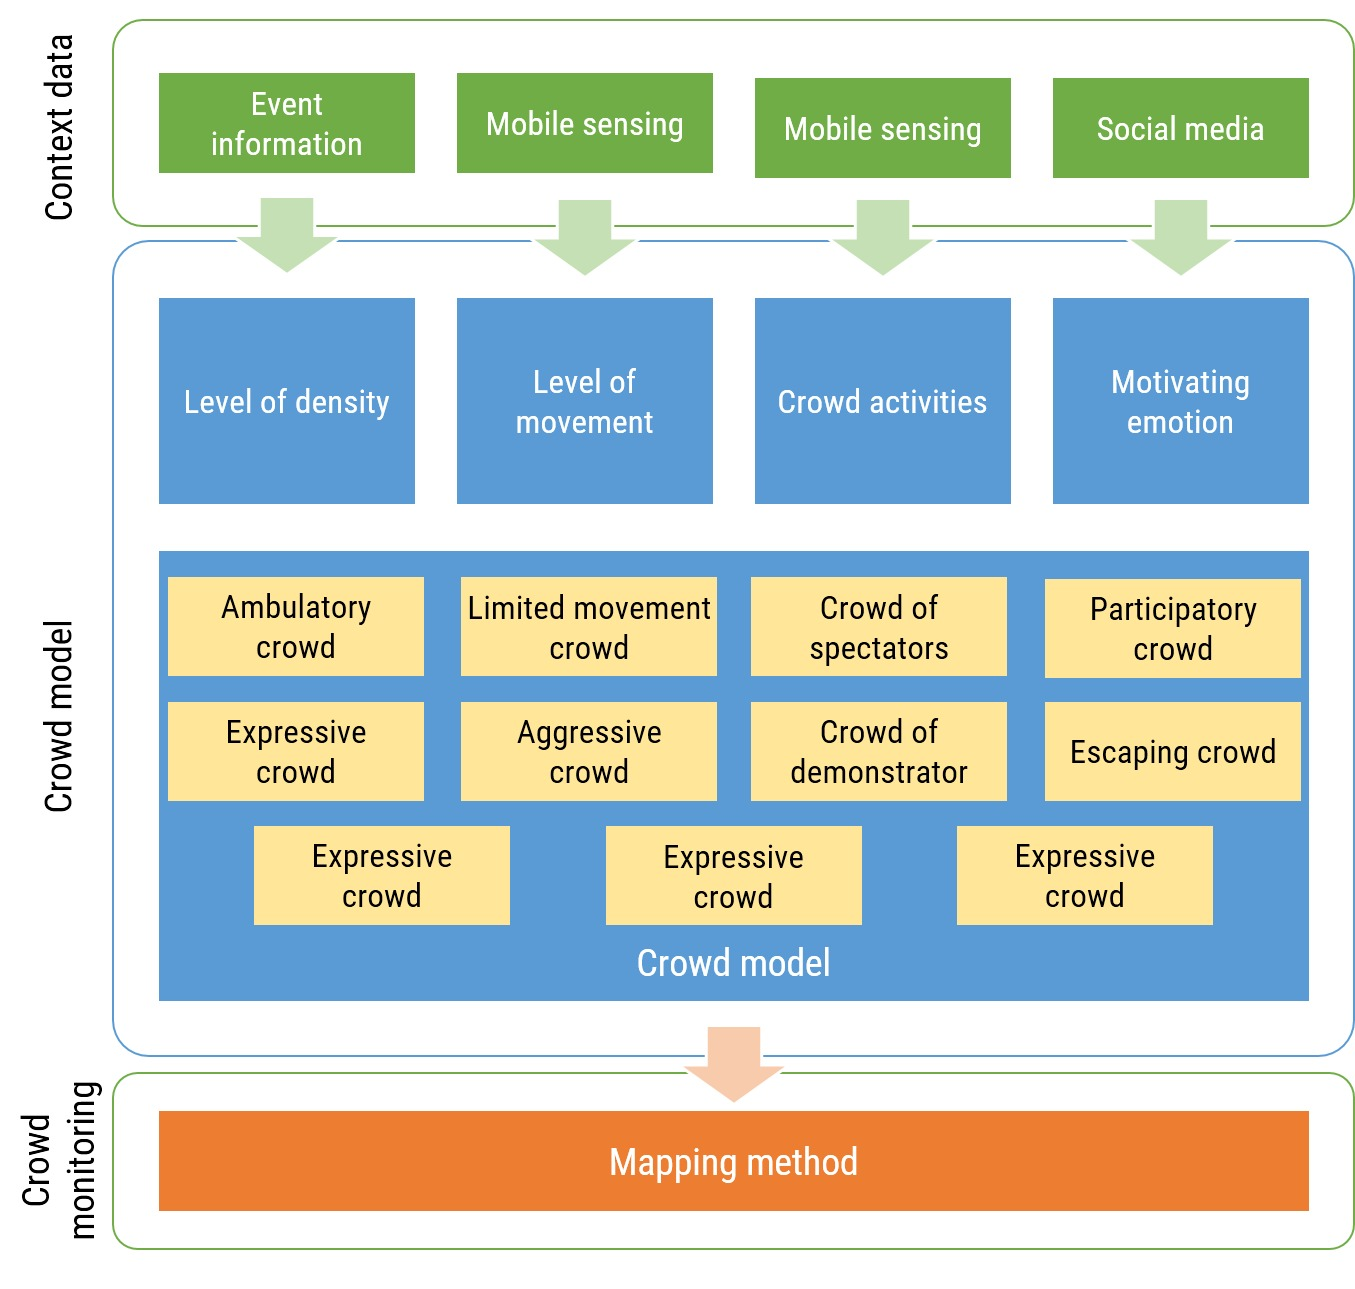
\includegraphics[width=1.0\textwidth]{FrameworkOverview}
\caption{An overview of the crowd monitoring framework using emotion analysis of social media}
\label{fig:frameworkOverview}
\end{figure}

\section{Context data}
The first component of the framework is context data component. In our proposed framework, contextual data is gathered from social media as the information source. Social media is the generic term referring to a wide range of Internet based tools that enable an user to create and share information with each other. These tools include social network services such as Facebook and Twitter, blogs, Internet forums and channels which has marked the beginning of Web 2.0. Unlike other traditional media such as newspaper or television, the content on social media is created by the users, or also known as user-generated content. In different social media, user-generated content can be in various formats such as text, image or video. Because of the fact that the content is being generated by the users themselves, social media is an effective source to obtain knowledge related to the users. In our domain and application of crowd monitoring, the knowledge that is interesting to collect is the emotional condition of the participants in the crowd.

Among these social media, Twitter is the most commonly used in researches because of its large volume of users and its public APIs which make the data highly accessible. The user-generated content is mostly text-based and in the form of a short message which has no more than 140 characters called tweet. Because of this length limit, a tweet is usually very simple in term of the meaning and each tweet focuses on expressing the idea of the author on one particular topic. This fact makes the semantic analysis of tweets more feasible than other content, for example, a long blog article.

A tweet might also contain information beyond the text. A significant number of tweets are geo-tagged, which means they are attached with location information when they are posted to Twitter. This location information can be in the form of exact 

Another useful information that might exist in a tweet is hashtags. Hashtags are created by the users, and usually they are put in a tweet to refer to the topic mentioned in the tweet. In some mass gathering events such as the Australia Open or music festivals, there are hashtags created for these particular events so that a user can put the hashtags into his tweet when mentioning about the events. Similarly to the geo-location, this information can also be used to filter for tweets belonging to a specific event.

Finally, using Twitter as the information source for crowd monitoring has some certain advantages. Firstly, the data can be collected in real-time, enabling the real-time monitoring which is an essential operation in emergency management because of the dynamic nature of a crowd that it can change from a calm type to an aggressive type \citep{Berlonghi1995}. Secondly, probing Twitter as a ``soft sensor'' does not require any pre-installed hardware or software on the participants, thus making it more feasible.

\section{Emotion Model}

As mentioned before, a crowd can be described as a form of collective behaviour of a group of people under the same motivation. In our framework, we emphasize on the emotional factor as the motivation of the behaviour in the crowd. Different emotions can consequently lead to different crowd behaviours. For example, if people in a riot is dominated by anger while on the other hand, fear might trigger a crushing crowd during an evacuation in a fire. Hence, an emotion model is essential to distinguish different emotions of the people in the crowd.

To represent the emotions of the participants in a crowd, our framework adapts Plutchik's wheel of emotion as the baseline for human basic emotions. Figure \ref{fig:emotionModel} illustrates the eight different basic emotions identified by Plutchik, consisting of anger, anticipation, joy, trust, fear, surprise, sadness and disgust. Each basic emotion has an opposite emotion, with which together forms a pair of contradictory emotions, such as sadness/joy or fear/anger. According to Plutchik's theory of emotion, other human emotions are either being a form of the lower and higher intensity of the eight emotions, or being a complex emotion composed of multiple basic emotions. For example, aggressiveness is a combination of anger and anticipation or remorse is a combination of sadness and disgust.

\begin{figure}[htbp!] 
\centering    
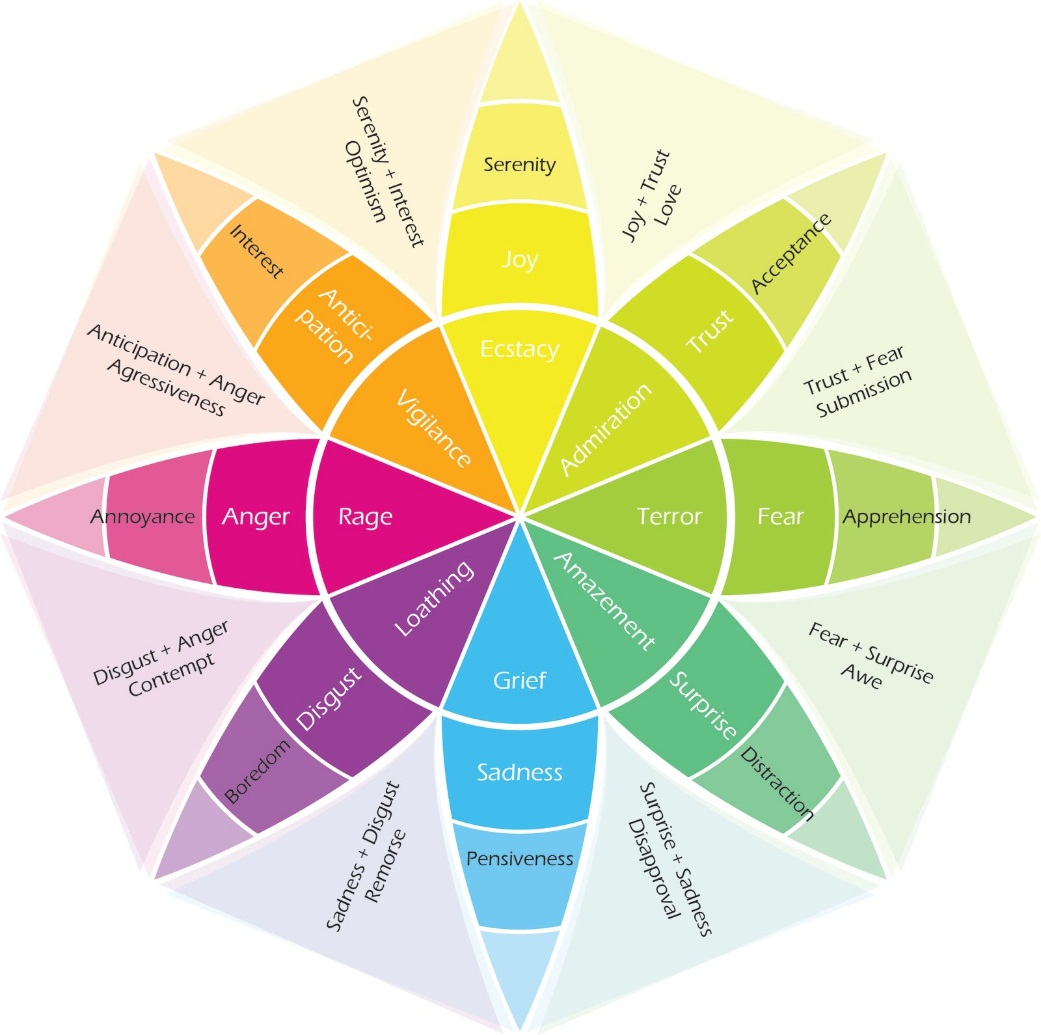
\includegraphics[width=1.0\textwidth]{PlutchikModel}
\caption{The Plutchik's wheel of emotions}
\label{fig:emotionModel}
\end{figure}

As can be seen from Figure \ref{fig:emotionModel}, the emotion wheel has eight wings representing eight basic human emotions. In each wing, the intensity of an emotion is increasing as it gets closer to the centre of the wheel. Adjacent emotions can mix and formula another advanced emotion as mentioned in the earlier examples. However in our approach, the emotion model only concentrates on the most basic eight emotions, hence it will not explore further into the intensity nor the mixture of these emotions.

\section{Emotion Analysis of Social Media}

As mentioned in the previous section, a tweet presents an opinion of the author, including the the emotion on a particular subject. By capturing the emotion expressed in the text, it is possible to infer the emotional state of the author. In our framework, a tweet can be considered as a raw context data that is collected from the information source while the emotion in the tweet is the high-level context data to be used in later crowd type classification. The emotion analysis component processes the raw data and produce the high-level context data.

The emotion analysis is based on a Bag-of-Word approach to classify 

\subsection{Emotion Word Lexicon}
This lexicon measures the association of a corpus of words with the eight emotions constructed by \citet{mohammad2014using}.

\subsection{Emotion Analysis}
We can detect the dominating emotion from a tweet using a bag of word approach. We then apply histogram with a specific time interval to measure the frequency of each emotion during that time frame.

\section{Crowd Model}

We use Berlonghi model

\section{Emotion - Crowd Type Mapping Model}

\subsection{From the individual emotion to the crowd emotions}
The emotion model mentioned in the previous section represent the emotional state of an individual. By performing the emotion analysis to a number of participants in a crowd, the general emotional states of the crowd can be inferred.

\subsection{Mapping crowd emotions to crowd type}
Table \ref{table:mappingEmotionCrowdType} presents our proposal for the mapping between each crowd type and eight basic emotions. Need to be revised, temporarily set as low or medium.

\begin{table}
\caption{Mapping between crowd types and emotions}
\label{table:mappingEmotionCrowdType}
\begin{tabular}{|p{2cm}|p{1.2cm}|p{1.2cm}|p{1.2cm}|p{1.2cm}|p{1.2cm}|p{1.2cm}|p{1.2cm}|p{1.2cm}|}
\hline
\textbf{Crowd type}	& \textbf{Anger}	& \textbf{Anticipation}	& \textbf{Joy} 	& \textbf{Trust}	& \textbf{Fear}	& \textbf{Surprise}	& \textbf{Sadness}	& \textbf{Disgust}	\\
\hline
Ambulatory			& low 				& medium				& medium		& medium			& low 			& low 				& medium			& low 		\\
\hline
Limited movement	& medium			& medium				& low 			& low 				& low 			& low 				& medium			& medium	\\
\hline
Spectator			& low 				& medium				& medium		& medium 			& low 			& medium			& low 				& low 		\\
\hline
Participatory		& low 				& medium				& medium		& medium			& low 			& low 				& low 				& low 		\\
\hline
Aggressive			& medium			& low 					& low 			& low 				& low 			& low 				& low 				& medium	\\
\hline
Demonstrator		& medium			& low 					& low 			& low 				& low 			& low 				& medium			& medium	\\
\hline
Escaping			& low 				& low 					& low 			& low 				& medium		& medium			& low 				& low 		\\
\hline
Dense				& medium			& low 					& low 			& low 				& medium		& medium			& low 				& medium	\\
\hline
Rushing				& medium			& low 					& low 			& low 				& low 			& low 				& low 				& medium	\\
\hline
Violent				& medium			& low 					& low 			& low 				& low 			& low 				& low 				& medium	\\
\hline
\end{tabular}
\end{table}

\section{Rule Based Reasoning}

\subsection{Fuzzifier}
We convert the numerical values of the frequency of appearance of an emotion into linguistic label: low, medium and high by applying following rules

if the value is below the low threshold of that emotion then the label is low
if the value is above the low threshold and below the high threshold then the label is medium
if the value is above the high threshold then the label is high

\subsection{Rule Repository}

list 11 rules here for 11 crowd types

\subsection{Inference Engine}

Fuzzy rule here and the mathematical formula here

\subsection{Output Processor}

the output is a vector of each crowd and its weight

\section{Conclusion}